% !TEX TS-program = pdflatex
% !TEX encoding = UTF-8 Unicode

% This is a simple template for a LaTeX document using the "article" class.
% See "book", "report", "letter" for other types of document.

\documentclass[12pt]{article} % use larger type; default would be 10pt

\usepackage[utf8]{inputenc} % set input encoding (not needed with XeLaTeX)

%%% Examples of Article customizations
% These packages are optional, depending whether you want the features they provide.
% See the LaTeX Companion or other references for full information.

%%% PAGE DIMENSIONS
\usepackage{geometry} % to change the page dimensions
\geometry{a4paper} % or letterpaper (US) or a5paper or....
\geometry{margin=1.2cm} % for example, change the margins to 2 inches all round
% \geometry{landscape} % set up the page for landscape
%   read geometry.pdf for detailed page layout information

\usepackage{graphicx} % support the \includegraphics command and options

% \usepackage[parfill]{parskip} % Activate to begin paragraphs with an empty line rather than an indent

%%% PACKAGES
\usepackage{booktabs} % for much better looking tables
\usepackage{array} % for better arrays (eg matrices) in maths
\usepackage{paralist} % very flexible & customisable lists (eg. enumerate/itemize, etc.)
\usepackage{verbatim} % adds environment for commenting out blocks of text & for better verbatim
\usepackage{subfig} % make it possible to include more than one captioned figure/table in a single float
% These packages are all incorporated in the memoir class to one degree or another...

%%% HEADERS & FOOTERS
\usepackage{fancyhdr} % This should be set AFTER setting up the page geometry
\pagestyle{empty} % options: empty , plain , fancy
\renewcommand{\headrulewidth}{0pt} % customise the layout...
%\lhead{}\chead{}\rhead{}
%\lfoot{}\cfoot{}\rfoot{}

%%% SECTION TITLE APPEARANCE
\usepackage{sectsty}
\allsectionsfont{\sffamily\mdseries\upshape} % (See the fntguide.pdf for font help)
% (This matches ConTeXt defaults)

%%% ToC (table of contents) APPEARANCE
\usepackage[nottoc,notlof,notlot]{tocbibind} % Put the bibliography in the ToC
\usepackage[titles,subfigure]{tocloft} % Alter the style of the Table of Contents
\renewcommand{\cftsecfont}{\rmfamily\mdseries\upshape}
\renewcommand{\cftsecpagefont}{\rmfamily\mdseries\upshape} % No bold!

%%% END Article customizations
\newcommand{\eqgood}{\overset{\surd}{=\joinrel=}}
\newcommand{\aufgabe}[2]{{\LARGE Algorithmen und Datenstrukturen Blatt #1 \underline{Aufgabe #2}}\\[3.5ex]  } 
\newcommand{\aufgabenstellung}[1]{\underline {#1}\\[2ex]}
\usepackage{amsmath}
\usepackage{amssymb}
%%% The "real" document content comes below...

\usepackage{color}
\definecolor{hellgruen}{rgb}{0.6,0.8,0.3}
\definecolor{dunkelgruen}{rgb}{0.3,0.7,0.4}
\begin{document}
\aufgabe{12}{1} 
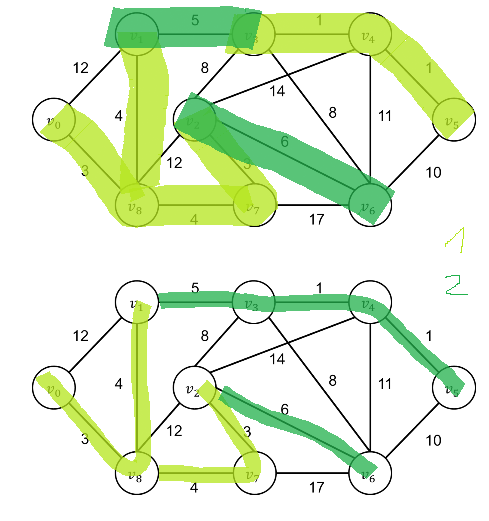
\includegraphics{Blatt12A1.png} \\
Die obere Grafik zeigt das Vorgehen mit Kruskals Algorithmus und die untere Grafik Prim. \\
Die Einzelschritte zu Kruskal: \\
\begin{tabular}{| r r | r | r | l | l |}
\hline
von & nach & Gewicht & Gesamtgewicht & Inselgroesse & Farbe in Grafik \\ \hline
$v_{3}$ & $v_{4}$ & $+1$ & $= 1$ & neue Insel & \textcolor{hellgruen}{hellgrün, oben rechts} \\ \hline
$v_{4}$ & $v_{5}$ & $+1$ & $= 2$ & Insel-Extension: 3 & \textcolor{hellgruen}{hellgrün, oben rechts} \\ \hline
$v_{0}$ & $v_{8}$ & $+3$ & $= 5$ & neue Insel & \textcolor{hellgruen}{hellgrün, unten links} \\ \hline
$v_{2}$ & $v_{7}$ & $+3$ & $= 8$ & neue Insel & \textcolor{hellgruen}{hellgrün, unten links} \\ \hline
$v_{1}$ & $v_{8}$ & $+4$ & $= 12$ & Insel-Extension: 3 & \textcolor{hellgruen}{hellgrün, unten links} \\ \hline
$v_{7}$ & $v_{8}$ & $+4$ & $= 16$ & Insel-Join: 3+2 = 5 & \textcolor{hellgruen}{hellgrün, unten links} \\ \hline
$v_{1}$ & $v_{3}$ & $+5$ & $= 21$ & Insel-Join: 5+3 = 8 & \textcolor{dunkelgruen}{dunkelgrün, oben} \\ \hline
$v_{2}$ & $v_{6}$ & $+6$ & $= 27$ & Insel-Extension: 9 & \textcolor{dunkelgruen}{dunkelgrün, unten} \\ \hline
\end{tabular} \\[1cm]
Die Einzelschritte zu Prim: \\
\begin{tabular}{| r r | r | r | lll | l |}
\hline 
von & nach & Gewicht & Gesamtgewicht & Heap-Root & Heap-Left & Heap-Right & Farbe \\ \hline
$v_{0}$ & $v_{8}$ & $+3$ & $= 3$ & $v_{1}: 4$ & $v_{2}: 12$ & $v_{7}: 4$ & \textcolor{hellgruen}{hellgrün} \\ \hline
$v_{8}$ & $v_{1}$ & $+4$ & $= 7$ & $v_{7}: 4$ & $v_{2}: 12$ & $v_{3}: 5$ & \textcolor{hellgruen}{hellgrün} \\ \hline
$v_{8}$ & $v_{7}$ & $+4$ & $= 11$ & $v_{2}: 3$ & $v_{3}: 5$ & $v_{6}: 17$ & \textcolor{hellgruen}{hellgrün} \\ \hline
$v_{7}$ & $v_{2}$ & $+3$ & $= 14$ & $v_{3}: 5$ & $v_{4}: 14$ & $v_{6}: 6$ & \textcolor{hellgruen}{hellgrün} \\ \hline
$v_{1}$ & $v_{3}$ & $+5$ & $= 19$ & $v_{4}: 1$ & $v_{6}: 6$ & -- & \textcolor{dunkelgruen}{dunkelgrün} \\ \hline
$v_{3}$ & $v_{4}$ & $+1$ & $= 20$ & $v_{5}: 1$ & $v_{6}: 6$ & -- & \textcolor{dunkelgruen}{dunkelgrün} \\ \hline
$v_{4}$ & $v_{5}$ & $+1$ & $= 21$ & $v_{6}: 6$ & -- & -- & \textcolor{dunkelgruen}{dunkelgrün} \\ \hline
$v_{2}$ & $v_{6}$ & $+6$ & $= 27$ & -- & -- & -- & \textcolor{dunkelgruen}{dunkelgrün} \\ \hline
\end{tabular}
\newpage
\aufgabe{12}{2}
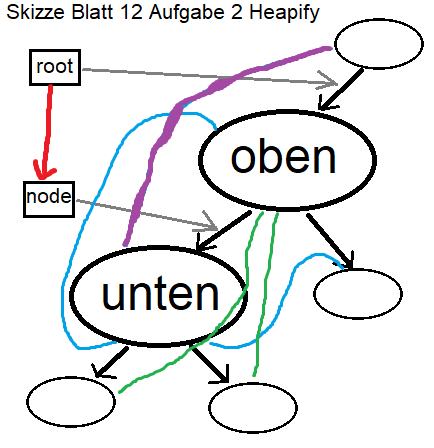
\includegraphics{Blatt12A2.png} \\
Die Grafik zeigt die Pointer-Umbiegungen beim Heapify. \\Details sind als Dokumentation im Quellcode angegeben. \\
\newpage
\aufgabe{12}{3}
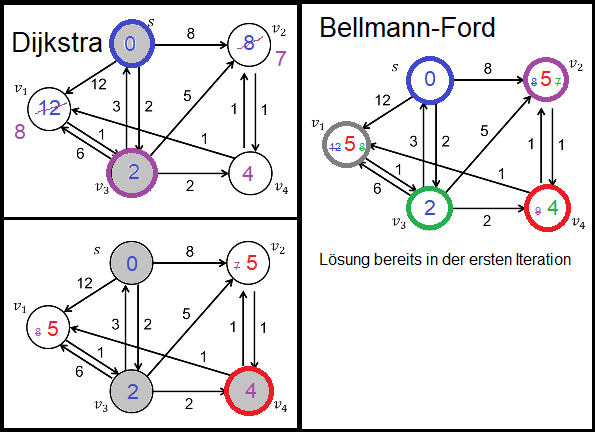
\includegraphics{Blatt12A3.png} \\
Dijksta-Algorithmus Step-by-Step: \\
\begin{tabular}{| r r r r r | r r r | l |}
\hline
$s$ & $v_{1}$ & $v_{2}$ & $v_{3}$ & $v_{4}$ & Heap-Root & Heap-Left & Heap-Right & Farbe \\ \hline \hline
$0$ & $12$ & $8$ & $2$ & $x$ & $v_{3}: 2$ & $v_{1}: 12$ & $v_{2}: 8$ & blau \\ 
 &  &  & \colorbox{black}{x} &  & $v_{2}: 8$ & $v_{1}: 12$ & -- &  \\ \hline
. & $8$ & $7$ &  & $4$ & $v_{4}: 4$ & $v_{1}: 8$ & $v_{2}: 7$ & lila \\ 
 &  &  &  & \colorbox{black}{x} & $v_{2}: 7$ & $v_{1}: 8$ & -- &  \\ \hline
 & $5$ & $5$ &  &  & $v_{1}: 5$ & $v_{2}: 5$ & -- & rot \\ 
 & \colorbox{black}{x} &  &  &  & $v_{2}: 5$ & -- & -- &  \\ \hline
\end{tabular}
\newpage
\aufgabe{12}{4a}
\aufgabenstellung{Warum kann Dijkstra nicht mit negativen Zahlen umgehen?}
Dijkstra markiert Knoten als erledigt, was bei negativen Gewichten falsch sein kann. \\
Lösung ist einfach: Die Erledigt-Markierungen einfach erst gar nicht implementieren. \\[2ex]
\- \dotfill \\[4ex] \hspace*{1em}
\aufgabe{12}{4b}
\aufgabenstellung{Warum kann man nicht das Minimum abziehen und so negative Zahlen eliminieren?}
Graph-Skizze: \\
$[S] -> [A] -> [B] -> [C] <- [S]$ \\[2ex]
Adjazenz-Kosten-Matrix (von Zeile nach Spalte):  \\[1ex]
\begin{tabular}{| l | l | l | l | l | l | l  l |} 
\hline
 & $S$ & $ A$ & $B$ & $C$ & $\sum$ & Ergebnis & \\ \hline
$S$ & x & $+6$ & - & $+4$ & $+0$ &  & \\ \hline
$A$ & - &  x & $-3$ & - & $+6$ &  & \\ \hline
$B$ & - &  - & x & $-2$ & $+3$ &  & \\ \hline
$C$ & - &  - & - & x & $+1$ & langer Weg ist besser (als 4) & \\ \hline
\end{tabular} \\[2ex]
Subtrahiert man nun überall das Minimum, also - -3, also +3, erhält man: \\[2ex]
\begin{tabular}{| l | l | l | l | l | l | l  l |} 
\hline
 & $S$ & $ A$ & $B$ & $C$ & $\sum$ & Ergebnis & \\ \hline
$S$ & x & $+9$ & - & $+7$ & $+0$ &  & \\ \hline
$A$ & - &  x & $+0$ & - & $+9$ &  & \\ \hline
$B$ & - &  - & x & $+1$ & $+9$ &  & \\ \hline
$C$ & - &  - & - & x & $+7$ & kurzer Weg ist besser (als 10) & \\ \hline
\end{tabular} \\[2ex]
Also: Modifizierter Algorithmus liefert anderes Ergebnis \\
Ergebnis: Algorithmus ist falsch.\\
\end{document}
